\documentclass[lualatex]{jlreq}
\usepackage{physics2}
\usephysicsmodule{ab}
\usepackage{tikz}
\usepackage{pgfplots}
\pgfplotsset{compat=1.18}

\title{LaTeX to DOCX Converter Sample}
\author{Sample Author}
\date{\today}

\begin{document}

\maketitle

\section{Introduction}

This document demonstrates the LaTeX to DOCX Converter with various features
including custom commands, TikZ diagrams, and data plots.

\section{Custom Commands}

Example using physics2 package's \verb|\ab()| command:

\[
\ab(x + y) = \left( x + y \right)
\]

Nested bracket example:

\[
\ab(\ab(a) + b) = \text{This kind of expression is also supported}
\]

\section{TikZ Diagrams}

\subsection{Basic Geometric Shapes}

\begin{figure}[h]
\centering
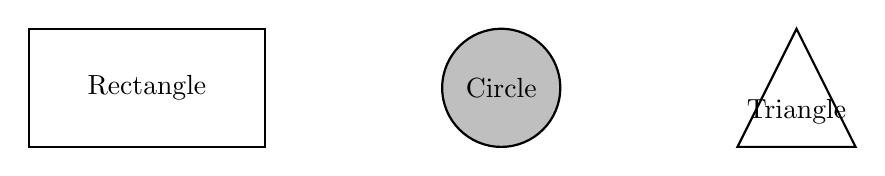
\begin{tikzpicture}[scale=1.5]
    % Rectangle
    \draw[thick] (0,0) rectangle (2,1);
    \node[anchor=center] at (1,0.5) {Rectangle};
    
    % Circle
    \draw[thick, fill=lightgray] (4,0.5) circle (0.5);
    \node[anchor=center] at (4,0.5) {Circle};
    
    % Triangle
    \draw[thick] (6,0) -- (7,0) -- (6.5,1) -- cycle;
    \node[anchor=center] at (6.5,0.3) {Triangle};
\end{tikzpicture}
\caption{Basic geometric shapes}
\label{fig:shapes}
\end{figure}

\subsection{Data Plotting}

\begin{figure}[h]
\centering
\begin{tikzpicture}
\begin{axis}[
    xlabel=X axis,
    ylabel=Y axis,
    width=8cm,
    height=6cm,
    grid=major,
    legend pos=north west
]
    \addplot[mark=*,blue] table {data/sample.dat};
    \addlegendentry{Sample data}
\end{axis}
\end{tikzpicture}
\caption{Data plot example}
\label{fig:plot}
\end{figure}

\section{Mathematical Equations}

Inline equation example: $E = mc^2$ is a famous formula.

Display equation example:

\begin{equation}
\frac{d}{dt}\ab(p(t)) = F(t)
\label{eq:newton}
\end{equation}

\section{Conclusion}

This sample demonstrates the conversion of LaTeX documents with
Japanese support, TikZ diagrams, and custom commands to Microsoft Word format.

\end{document}
